% A template for Yale-NUS MCS Capstone by Chong Woon Han (Class of 2018)
% Loosely based off the instructions in the Capstone Instructions Word Document that was circulated in AY 2017/2018

\documentclass[12pt]{article}
\usepackage{blindtext}
\usepackage{titlesec}
\usepackage[utf8]{inputenc}
\usepackage{geometry}
\geometry{a4paper,top=3cm,bottom=3cm,right=3cm,left=4cm}
% \setcounter{section}{-1}
\usepackage{setspace}
\usepackage{amsmath}
\usepackage{appendix}
\usepackage{pdfpages}
\usepackage{graphicx}
\usepackage{float}
\graphicspath{{images/}} % define the relative directory where \includegraphics{} will insert images from

%------ For bibliography -------
\usepackage[sorting=none]{biblatex}
\addbibresource{cwh_capstone_biblio.bib} % Put your .bib file here for your bibliography
% You can refer to the example .bib file I included. If you use Mendeley, it has a pretty cool feature where you can right click a reference to generate a bibtex entry like this:
% right-click the reference > Copy As > BibText Entry
% Then you just paste it into the .bib file! ezpz! If only I could say the same for my Capstone...

%----- For code snippets ------
\usepackage{minted} % for code
\usepackage{xcolor}
\definecolor{light-gray}{gray}{0.95}

%------------- TITLE PAGE ------------
% I didn't actually use this because in my year we had to use a specific cover page, which I inserted as a PDF
\title{\textbf{Your title here}}
\author{\textbf{Your name here}\\
Your Student ID here\\
\\
Capstone Final Report for BSc (Honours) in\\
Mathematical, Computational and Statistical Science\\
2018}
\date{}

% ---------- DOCUMENT ------------
\begin{document}
\begin{spacing}{1.9}

% In my year, we were given a Word Document which had a cover page design we had to follow. I exported that page as a pdf and included it here:

\includepdf[pages={1}]{Final-Capstone-Title-Page-BSc.pdf}
% If that's not necessary for you, then just un-comment the following line:
% \maketitle

\clearpage

% You can also use \includepdf to include the consent form (if applicable). Please be nice to your supervisor and ask for their signature long before the deadline
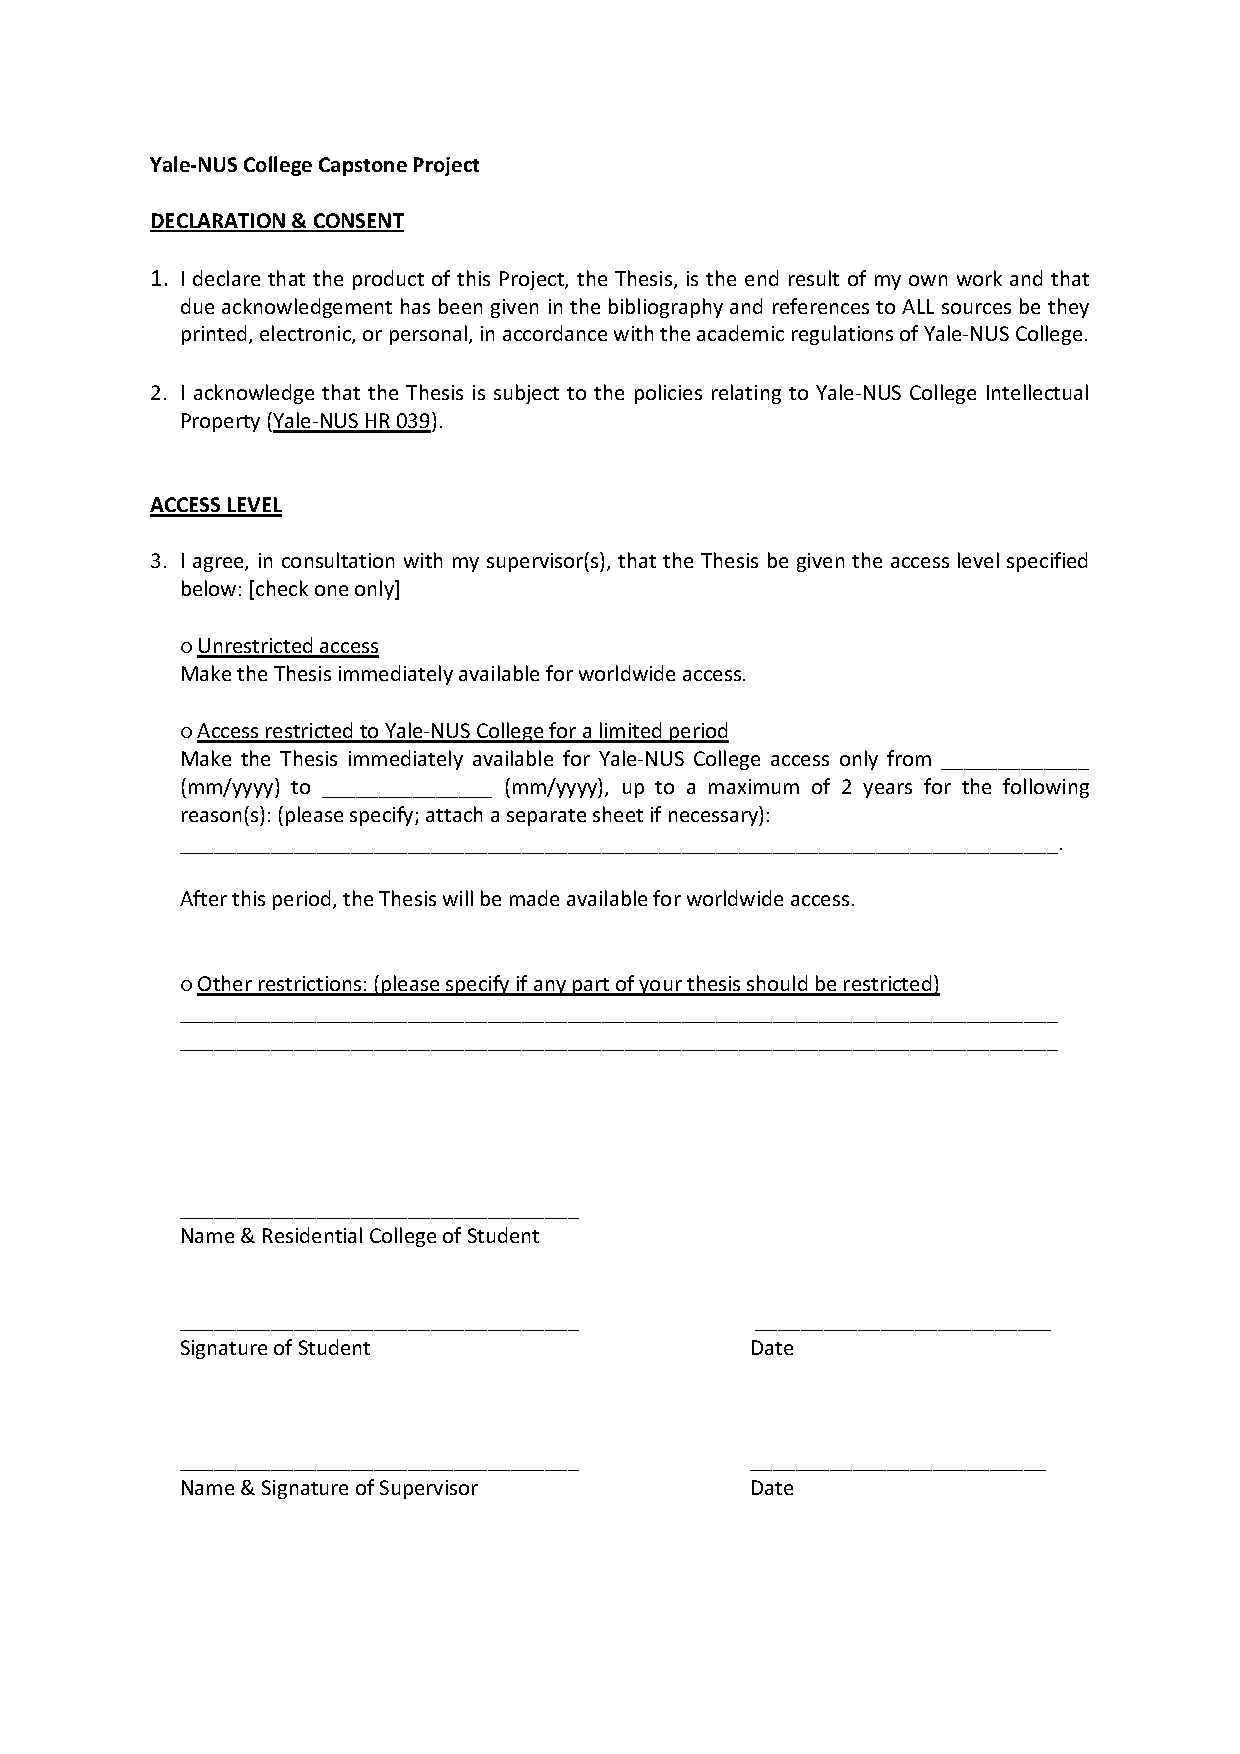
\includepdf[pages={1}]{CapstoneDeclarationConsentForm.pdf}

\clearpage

\section*{Acknowledgements}
Your acknowledgements here. Don't forget to acknowledge your Significant Other (if applicable) or they will leave you and go back to Canada

\section*{Summary}
Your summary here

\section*{Statement of Author's Contributions}
Your contributions here (mine was completely empty. jk)

\clearpage

% This will automatically create a table of contents as long as you use the \section{} \subsection{} \subsubsection{} features 
\tableofcontents

\clearpage

% ------------------------------------------ [EXAMPLE COMMENT SECTION TO INCREASE YOUR QOL WHEN READING YOUR LATEX CODE] ----------------------------------------------------

\section{List of Tables}

% My "tables" were actually png files inserted as figures using the following code:
% Please don't even try creating tables in Latex - even the legendary Sean Saito (Class of 2017) senpai hates doing it
\begin{figure}[H]
    \centering
    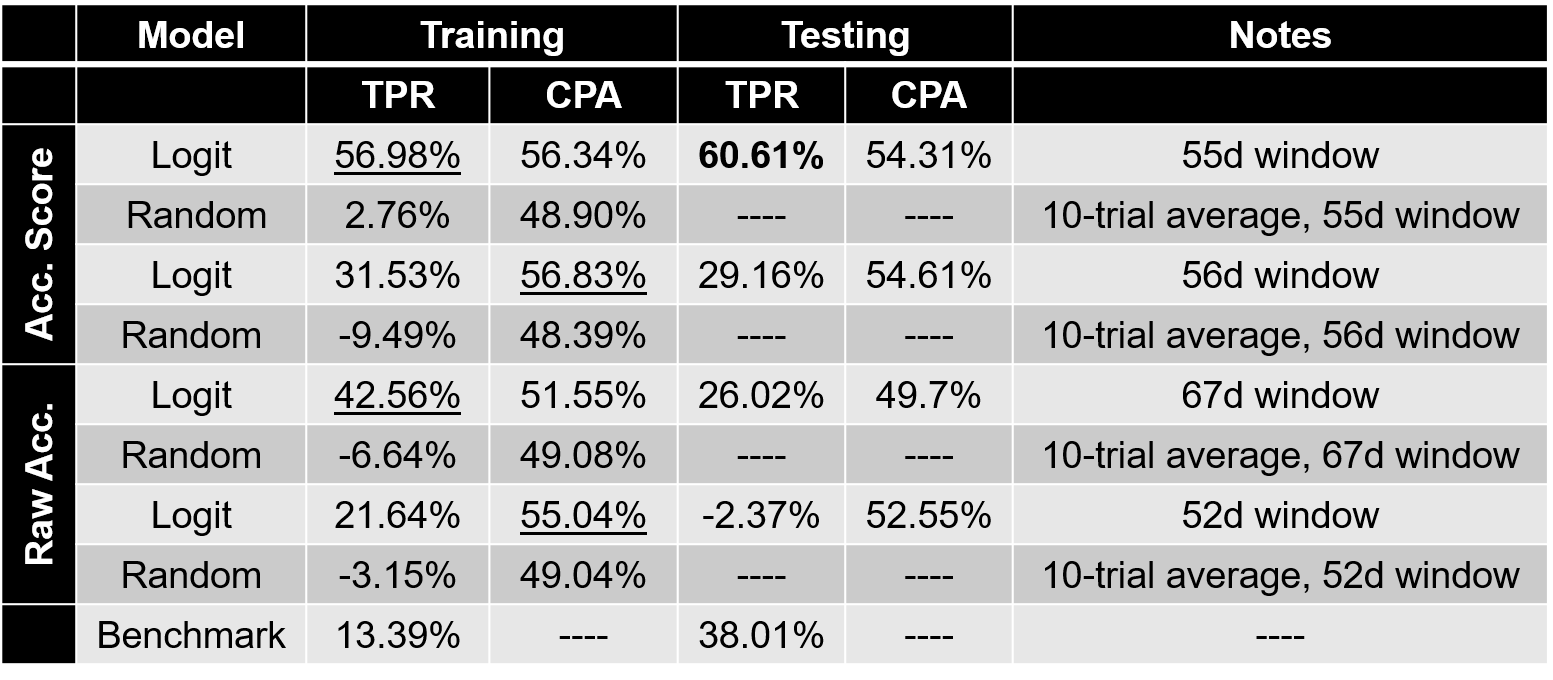
\includegraphics[scale=0.50]{table_logit_random.png}
    \caption{Your table caption here}
    \label{tab:table_logit_random}
\end{figure}

\section{List of Figures}

% Same thing if you want to add actual figures
\begin{figure}[H]
    \centering
    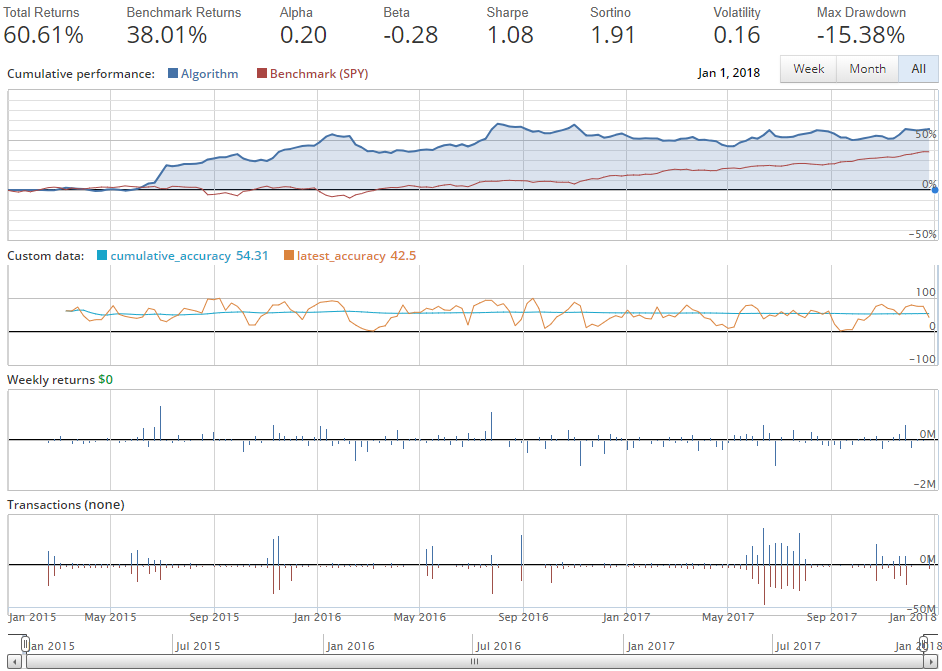
\includegraphics[scale=0.55]{results_logit.png}
    \caption{Your figure caption here}
    \label{fig:results_logit}
\end{figure}

\section{Chapters and Sections}
\subsection{Introduction}
Your introduction here with a citation \cite{Atsalakis}. 
% observe that the argument used in \cite{} is the first argument/field in each item in the .bib file

% -------------------------- Subsection 1 ----------------------------
\subsection{Subsection 1}
    \subsubsection{Sub-subsection 1}
    bLoCk ChAiN
    
    \subsubsection{Sub-subsection 2}
    mAcHiNe LeArNiNg
    
% The indentation does not affect the output - it is merely for readability of code    
    

% -------------------------- Subsection 2 ----------------------------    
\subsection{Subsection 2}
This is how to put short code snippets like \mintinline{python}{foobar.method()}

\section{Results and Discussion}
This is the part where I pretended I knew what my results meant

\section{Conclusion}
Conclusion here

% Your biblio
\section{References}
\printbibliography

% Example appendix where you can put anything you want, including your code
\appendix
\section{Appendices}
% Here's how you insert a whole chunk of code (you can use it in the Capstone itself too)
\begin{minted}[bgcolor=light-gray,fontsize=\footnotesize,baselinestretch=1.2,linenos,breaklines]{python}
"""
Example Python Code
"""

def doCapstone():
    while True:
        suffer()
\end{minted}

\end{spacing}
\end{document}

% All the best for your Capstone!
